\section{Interface}

Notre application se présente de la manière suivante :\\
une barre de menu situé au nord de la fenêtre vous permettra de choisir 
une action à réaliser parmi toutes les fonctionnalités qui vous sont proposés.\\
\\
La grille de sudoku occupe le centre de notre application et se retrouve accompagnée 
d'une colonne, à l'est de la fenêtre, vous permettant de sélectionner 
parmi des boutons raccourcis, les fonctionnalités les plus utilisés tel défaire, 
refaire une action, demander un indice, réinitialiser la grille etc, puis, 
une zone d'aide, situé en bas de la grille.\\

Il vous est également possible d'utiliser votre clavier afin de profiter 
des fonctionnalités que vous offre notre application.\\
Pour ce faire, il vous suffit de saisir la combinaison appropriée, combinaison 
que vous pourrez retrouver en consultant les listes des fonctionnalités disponibles dans le menu, 
au nord de l'application, où coïncide chaque fonctionnalité avec sa combinaison 
de la forme CTRL+LETTRE, qu'il vous suffit d'utiliser en appuyant simultanément 
sur la touche contrôle et la lettre correspondante à l'action souhaîtée. \\

Pour ajouter/retirer des possibilités dans la grille, il vous suffit d'utiliser 
le bouton droit de la souris tandis que pour ajouter/retirer des candidats, il 
faudra utiliser le bouton gauche de votre souris.

\begin{figure}[ht]
  \caption{\label{annexe6} interface sudoku}
  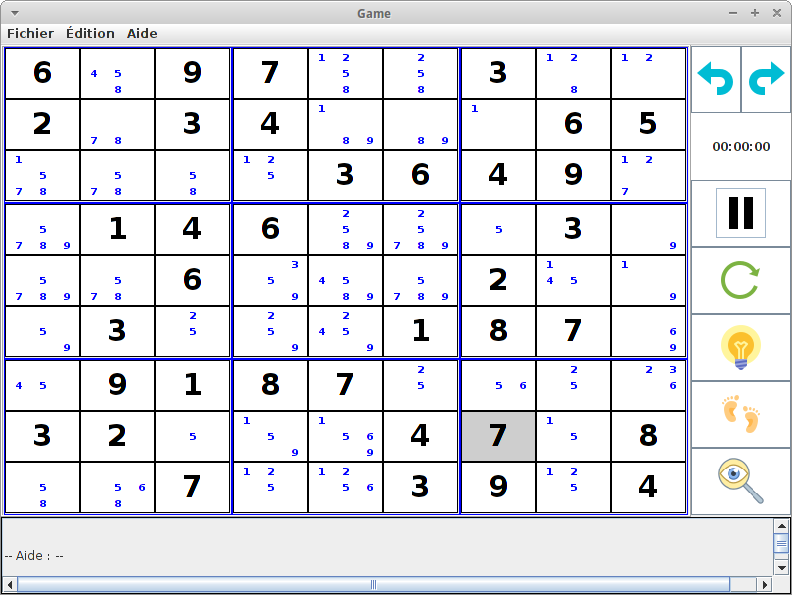
\includegraphics [width=130mm]{images/interface.png} \\[0.5cm]
\end{figure}

\newpage
\section{Difficultés rencontrées}
Lors de la conception de notre projet, nous avons rencontrés quelques difficultés :
\begin{itemize}
 \item gestion du temps, où chaque semaine, nous nous fixions des objectifs à atteindre,
 \item utilisation et prise en main du logiciel git et du site 
	    \href{https://github.com/yuki1996/Sudoku}{github.com}, 
 \item respect des demandes de la part du client, 
 \item incompatibilité/réajustement lors de réunion de différents travaux des membres du groupe
\end{itemize}


\section{Conclusion}
Ce projet nous a apporté une grande expérience car il s'agit 
de notre premier ``gros'' projet en équipe de plus de deux personnes.

Afin de réaliser un travail commun, nous avons opté pour un service 
de gestion de développement de logiciels, utilisant le logiciel 
de gestion de versions Git ainsi que le service web d'hébergement \url{https://github.com/}.

Ce dernier fut pour nous d'une grande aide, ce fut une toute nouvelle façon de 
procéder que nous a donné comme opportunité ce projet même si la prise en main 
fut assez compliqué.

Pour finir, ce projet fut pour nous très enrichissant car il nous a permi de réunir
l'ensemble de nos connaissances au sein d'un même projet. Nous avons fait le choix 
de développer notre application dans le langage de programmation Java, qui est un langage
très intéressant pour les développements d'applications graphiques.

\section{Annexes}

\begin{figure}[ht]
  \caption{\label{annexe7} Diagramme model}
  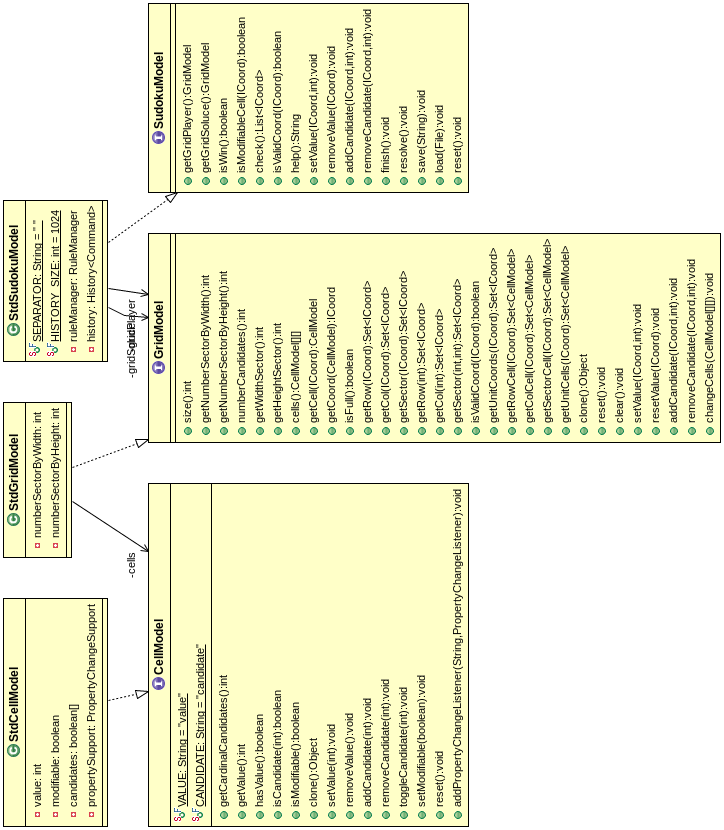
\includegraphics [width=160mm]{images/model.png} \\[0.5cm]
\end{figure}

\begin{figure}[ht]
  \caption{\label{annexe8} Diagramme history}
  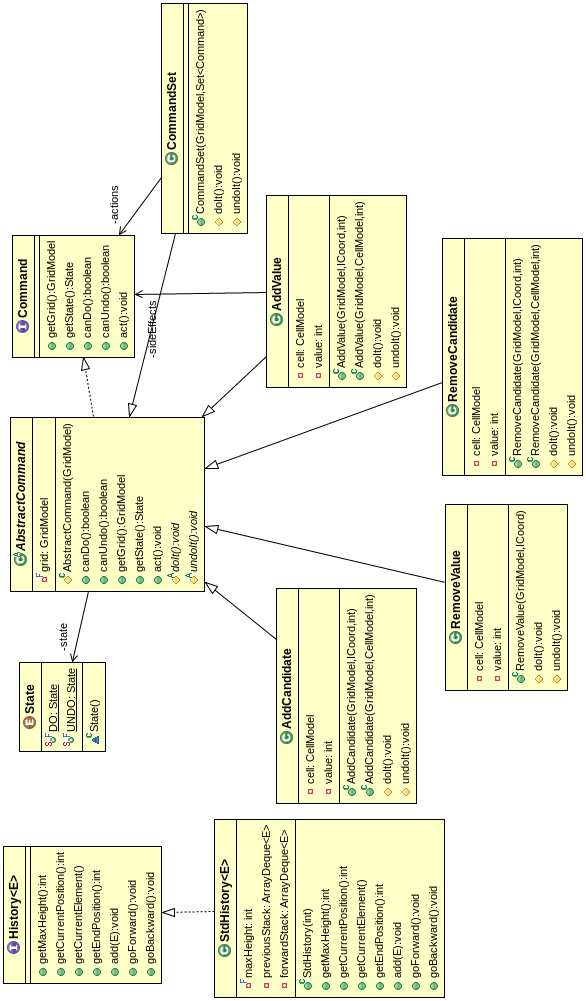
\includegraphics [width=140mm]{images/history.png} \\[0.5cm]
\end{figure}

\begin{figure}[ht]
  \caption{\label{annexe9} Diagramme heuristic}
  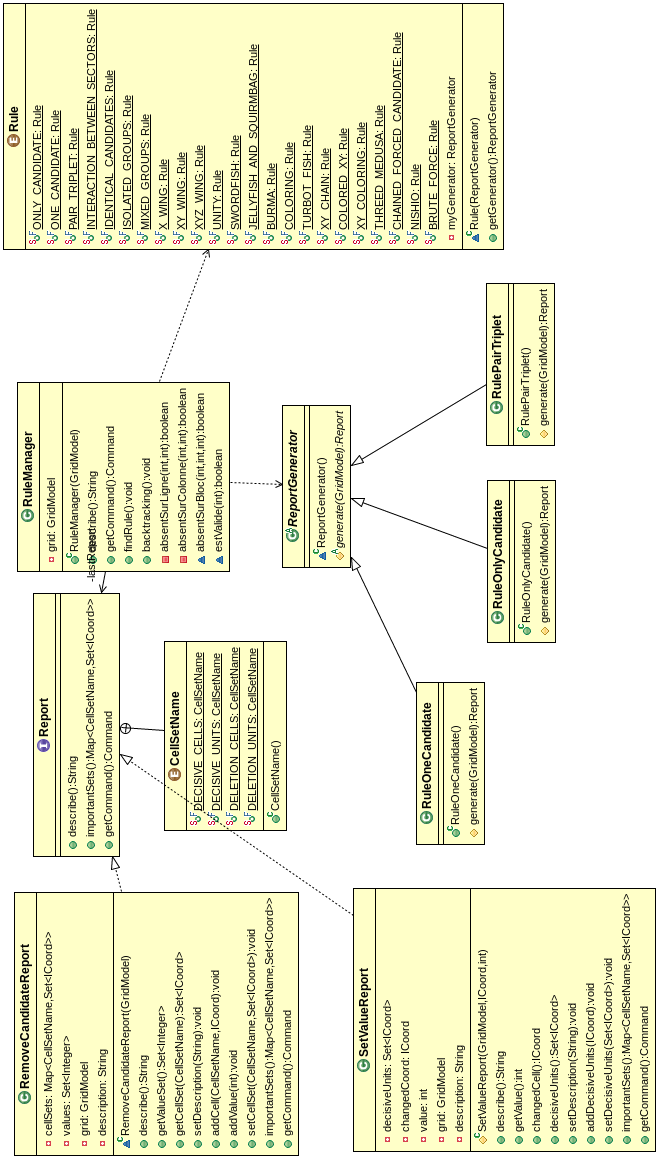
\includegraphics [width=140mm]{images/heuristic.png} \\[0.5cm]
\end{figure}

